\subsection{Infinite Series and Summability}


This subsection treats a series as a sequence of partial sums, so convergence and tests such as comparison, condensation, root, ratio, summation by parts, absolute convergence, products, rearrangements, and double sums lean on Definition \ref{def:sequence-convergence-metric} and Theorem \ref{thm:cauchy-convergence-criterion}. Power-series radius material is developed later in Definition \ref{def:power-series-radius-basic}.

\begin{definition} \label{def:series-core-definitions-source-todo}\label{def:series-and-partial-sums} \hlt{Series and Partial Sums}\\
Let $(a_n)$ be a complex sequence, and for $p\leq q$ put $\sum\limits_{n=p}^{q}a_n\defeq a_p+a_{p+1}+\cdots+a_q$.\\
The index $n$ in the displayed finite sum is a bound variable, in the sense of Principle \ref{princ:well-formed-statements-and-bound-variables}; it may be renamed when its scope is unchanged.\\
The \hlt{series} $\sum_{n=1}^{\infty}a_n$ (or $a_1+a_2+\cdots$) is the partial-sum sequence $s_n\defeq\sum\limits_{k=1}^{n}a_k$. If $s_n\to s$, then $\sum\limits_{n=1}^{\infty}a_n=s$ and series \hlt{converges}; otherwise it \hlt{diverges}. The same convention applies to series starting at $n=0$.
\end{definition}


\begin{motivation} \label{mot:partial-sums-remember-order} \hlt{Partial Sums Remember Order}\\
An infinite sum is a limit of partial sums. For alternating harmonic series, odd and even partial sums approach the same value from opposite sides; see Corollary \ref{cor:alternating-series-test} and Theorem \ref{thm:absolute-convergence-rearrangements}.
\end{motivation}

\begin{perspective} \label{per:formal-series-algebra-needs-convergence} \hlt{Formal Algebra Needs Convergence}\\
Finite sums are algebraic; infinite sums are partial-sum limits. Algebraic manipulations are justified only by convergence control, as in Theorem \ref{thm:series-cauchy-criterion}, Corollary \ref{cor:series-terms-tend-to-zero}, and Theorems \ref{thm:mertens-cauchy-product}, \ref{thm:absolute-convergence-rearrangements}.\\
\hlt{Key Insight}: The symbol $\sum_{n=1}^{\infty}$ is a limit claim before it is an algebraic object.
\end{perspective}

\begin{theorem} \label{thm:series-cauchy-criterion}\label{thm:series-main-results-source-todo} \hlt{Cauchy Criterion for Series}\\
The series $\sum a_n$ converges if and only if $\forall \varepsilon>0$ $\exists$ an integer $N$ s.t. $m\geq n\geq N$ implies $\abs{\sum\limits_{k=n}^{m}a_k}\leq\varepsilon$.
\begin{proof}
\begin{enumerate}[label=\roman*.]
\setlength{\itemsep}{0pt}
\item[$(\Rightarrow)$] If $s_n\defeq\sum\limits_{k=1}^{n}a_k$ converges, then $(s_n)$ is Cauchy. Thus, for $m\geq n$ large enough, $\abs{\sum\limits_{k=n}^{m}a_k}=\abs{s_m-s_{n-1}}\leq\varepsilon$.
\item[$(\Leftarrow)$] The tail condition gives, for $m>n$ large enough, $\abs{s_m-s_n}=\abs{\sum\limits_{k=n+1}^{m}a_k}\leq\varepsilon$.\\
Hence $(s_n)$ is Cauchy and converges by Theorem \ref{thm:cauchy-convergence-criterion}.
\end{enumerate}
\hlt{Structural Commentary}: A series converges exactly when all sufficiently late finite tails are small.\\
\hlt{Key Insight}: The Cauchy test measures tails, not the eventual value of the sum.
\end{proof}
\end{theorem}

\begin{corollary} \label{cor:series-terms-tend-to-zero} \hlt{Terms of a Convergent Series Tend to Zero}\\
If $\sum a_n$ converges, then $a_n\to0$.
\begin{proof}
Let $\varepsilon>0$. By Theorem \ref{thm:series-cauchy-criterion}, there is $N$ such that $m\geq n\geq N$ implies $\abs{\sum_{k=n}^{m}a_k}\leq\varepsilon$.\\
Taking $m=n$ gives $\abs{a_n}\leq\varepsilon$ for all $n\geq N$, hence $a_n\to0$.\\
\hlt{Structural Commentary}: A single term is the shortest possible tail.\\
\hlt{Key Insight}: The condition $a_n\to0$ is necessary, but not sufficient for convergence.
\end{proof}
\end{corollary}

\begin{theorem} \label{thm:nonnegative-series-bounded-partial-sums} \hlt{Nonnegative Series and Bounded Partial Sums}\\
A series of nonnegative real terms converges if and only if its partial sums form a bounded sequence.
\begin{proof}
\begin{enumerate}[label=\roman*.]
\setlength{\itemsep}{0pt}
\item[$(\Rightarrow)$] Every convergent sequence is bounded, so the partial sums are bounded.
\item[$(\Leftarrow)$] Since $a_n\geq0$, $s_n=\sum\limits_{k=1}^{n}a_k$ increases; if bounded, it converges by Theorem \ref{thm:monotone-convergence}.
\end{enumerate}
\hlt{Structural Commentary}: Nonnegative series replace cancellation by monotonicity.\\
\hlt{Key Insight}: For nonnegative terms, convergence is exactly bounded accumulation.
\end{proof}
\end{theorem}

\begin{theorem} \label{thm:series-comparison-test} \hlt{Comparison Test}
\begin{enumerate}[label=(\roman*)]
\setlength{\itemsep}{0pt}
\item If $\abs{a_n}\leq c_n$ for $n\geq N_0$, and if $\sum c_n$ converges, then $\sum a_n$ converges.
\item If $a_n\geq d_n\geq0$ for $n\geq N_0$, and if $\sum d_n$ diverges, then $\sum a_n$ diverges.
\end{enumerate}
\begin{proof}
\begin{enumerate}[label=(\roman*)]
\setlength{\itemsep}{0pt}
\item Given $\varepsilon>0$, choose $N\geq N_0$ so that $m\geq n\geq N$ implies $\sum_{k=n}^{m}c_k\leq\varepsilon$.\\
Then $\abs{\sum\limits_{k=n}^{m}a_k}\leq\sum_{k=n}^{m}\abs{a_k}\leq\sum\limits_{k=n}^{m}c_k\leq\varepsilon$, so Theorem \ref{thm:series-cauchy-criterion} applies.
\item If $\sum a_n$ converged, then (i) applied to $d_n\leq a_n$ would force $\sum d_n$ to converge, a contradiction.
\end{enumerate}
\hlt{Structural Commentary}: Absolute tail domination transfers Cauchy convergence.\\
\hlt{Key Insight}: Comparison is a tail test; finitely many early terms do not matter.
\end{proof}
\end{theorem}

\begin{theorem} \label{thm:geometric-series-nonnegative} \hlt{Geometric Series}\\
If $0\leq x<1$, then $\sum\limits_{n=0}^{\infty}x^n=\frac{1}{1-x}$. If $x\geq1$, the series diverges.
\begin{proof}
For $x\neq1$, $\sum\limits_{k=0}^{n}x^k=\frac{1-x^{n+1}}{1-x}$. Let $n\to\infty$ and use Theorem \ref{thm:special-sequence-limits}.\\
If $x=1$, the partial sums are $n+1$, so they diverge.\\
\hlt{Structural Commentary}: The finite geometric identity converts convergence into the limit of $x^{n+1}$.\\
\hlt{Key Insight}: The geometric series is the model comparison series for ratio-like decay.
\end{proof}
\end{theorem}

\begin{definition} \label{def:real-decimal-as-series} \hlt{Real Decimals as Series}\\
For digits $b_N,\ldots,b_0,a_1,a_2,\ldots\in\{0,\ldots,9\}$, with $b_N\neq0$ unless the integer part is $0$,\\
$b_N\cdots b_0.a_1a_2\cdots \defeq \sum\limits_{i=0}^{N}b_i10^i+\sum\limits_{j=1}^{\infty}a_j10^{-j}$. The fractional series converges absolutely since $0\leq a_j10^{-j}\leq9\cdot10^{-j}$ and $\sum 9\cdot10^{-j}$ is geometric. A minus sign denotes the negative of this value.
\end{definition}

\begin{proposition} \label{prop:decimal-terminal-nine-nonuniqueness} \hlt{Terminal Nines Are Nonunique}\\
The same real number can have two decimal representations: $1.000\ldots=0.999\ldots$.
\begin{proof}
By Definition \ref{def:real-decimal-as-series} and Theorem \ref{thm:geometric-series-nonnegative}, $1.000\ldots=1$; $0.999\ldots=\sum\limits_{j=1}^{\infty}9\cdot10^{-j} =9\cdot\frac{10^{-1}}{1-10^{-1}}=1$.\\
\hlt{Structural Commentary}: The two digit strings have the same partial-sum limit.\\
\hlt{Key Insight}: Uniqueness requires excluding terminal $9$ tails.
\end{proof}
\end{proposition}

\begin{perspective} \label{per:decimal-expansions-as-series} \hlt{Decimal Expansions Are Series}\\
Proposition \ref{prop:decimal-truncations-squeeze-real} gives decimal truncations that converge to a real number, while Definition \ref{def:real-decimal-as-series} interprets the infinite digit string as a series. Proposition \ref{prop:decimal-terminal-nine-nonuniqueness} explains the standard terminal-$9$ ambiguity.
\end{perspective}

\begin{theorem} \label{thm:cauchy-condensation-test} \hlt{Cauchy Condensation Test}\\
Suppose $a_1\geq a_2\geq a_3\geq\cdots\geq0$. Then $\sum_{n=1}^{\infty}a_n$ converges if and only if $\sum\limits_{k=0}^{\infty}2^k a_{2^k}$ converges.
\begin{proof}
Let $s_n\defeq a_1+\cdots+a_n$ and $t_k\defeq a_1+2a_2+\cdots+2^k a_{2^k}$.\\
If $n<2^k$, then grouping by dyadic blocks gives $s_n\leq a_1+(a_2+a_3)+\cdots+(a_{2^k}+\cdots+a_{2^{k+1}-1})\leq t_k$.\\
If $n>2^k$, grouping from the other side gives $2s_n\geq t_k$. Hence the nonnegative partial sums $(s_n)$ and $(t_k)$ are either both bounded or both unbounded; apply Theorem \ref{thm:nonnegative-series-bounded-partial-sums}.\\
\hlt{Structural Commentary}: Monotonicity lets dyadic blocks be compared to their endpoint terms.\\
\hlt{Key Insight}: A sparse dyadic subsequence detects the whole monotone nonnegative series.
\end{proof}
\end{theorem}

\begin{corollary} \label{cor:p-series-test} \hlt{$p$-Series Test}\\
The series $\sum\limits_{n=1}^{\infty}\frac{1}{n^p}$ converges if $p>1$ and diverges if $p\leq1$.
\begin{proof}
If $p\leq0$, the terms do not tend to $0$, so Corollary \ref{cor:series-terms-tend-to-zero} gives divergence.\\
If $p>0$, Theorem \ref{thm:cauchy-condensation-test} reduces the question to $\sum\limits_{k=0}^{\infty}2^k\frac{1}{(2^k)^p}=\sum\limits_{k=0}^{\infty}2^{(1-p)k}$.\\
This geometric series converges exactly when $2^{1-p}<1$, i.e. $p>1$, by Theorem \ref{thm:geometric-series-nonnegative}.\\
\hlt{Structural Commentary}: Condensation turns powers of $n$ into powers of $2$.\\
\hlt{Key Insight}: The boundary is $p=1$ because the condensed ratio is $2^{1-p}$.
\end{proof}
\end{corollary}

\begin{figure}[H]
  \centering
  \begin{tikzpicture}[
  x=0.78cm,
  y=0.72cm,
  >=Stealth,
  every node/.style={font=\scriptsize},
  axis/.style={->, black!55, line width=0.45pt},
  curve/.style={black!85, line width=0.9pt},
  upper/.style={draw=black!55, line width=0.45pt},
  lower/.style={fill=gray!18, draw=black!55, line width=0.45pt},
  guide/.style={black!18, dashed, line width=0.35pt}
]
  \draw[axis] (-0.25,0) -- (5.65,0) node[right] {$x$};
  \draw[axis] (0,-0.15) -- (0,3.20);

  \foreach \x in {0,1,2,3,4,5} {
    \draw[guide] (\x,0) -- (\x,3.0);
  }
  \foreach \x/\lab in {0/$N$,1/$N+1$,4/$M$,5/$M+1$} {
    \node[below] at (\x,0) {\lab};
  }
  \node[below] at (2.55,0) {$\cdots$};

  \foreach \xl/\xr in {0/1,1/2,2/3,3/4,4/5} {
    \pgfmathsetmacro{\hleft}{2.55/(1+0.42*\xl)+0.35}
    \pgfmathsetmacro{\hright}{2.55/(1+0.42*\xr)+0.35}
    \draw[lower] (\xl,0) rectangle (\xr,\hright);
    \draw[upper] (\xl,0) rectangle (\xr,\hleft);
  }

  \draw[curve, domain=0:5.15, samples=120]
    plot (\x,{2.55/(1+0.42*\x)+0.35}) node[right] {$f$};
\end{tikzpicture}

  \caption{Left and right endpoint estimates for decreasing $f\geq0$.}
  \label{fig:integral-test-step-functions}
\end{figure}

\begin{theorem} \label{thm:integral-test-series} \hlt{Integral Test}\\
Let $N\in\N$ and let $f:[N,\infty)\to[0,\infty)$ be decreasing and Riemann integrable on compact subintervals.\\
Then $\sum\limits_{k=N}^{\infty}f(k)$ converges iff $\int_N^\infty f(x)\,dx$ converges.\\
For $M\geq N$, $\int_N^{M+1} f(x)\,dx \leq \sum\limits_{k=N}^{M}f(k) \leq f(N)+\int_N^M f(x)\,dx$.
\begin{proof}
For a monotone function, compact-subinterval Riemann integrability follows from Theorem \ref{thm:monotone-functions-integrable-continuous-integrator} with $\alpha(x)=x$; it is kept in the statement to make the improper-integral dependency explicit.
\begin{enumerate}[label=\roman*.]
\setlength{\itemsep}{0pt}
\item[$(\Rightarrow)$] For $x\in[k,k+1]$, monotonicity gives $f(x)\leq f(k)$. Hence $\int_N^{M+1}f(x)\,dx\leq\sum_{k=N}^{M}f(k)$. If the series converges, these truncations are bounded, so $\int_N^\infty f$ converges by Theorem \ref{thm:nonnegative-improper-integral-supremum}.
\item[$(\Leftarrow)$] For $k\geq N+1$ and $x\in[k-1,k]$, monotonicity gives $f(k)\leq f(x)$. Hence $\sum_{k=N}^{M}f(k)\leq f(N)+\int_N^M f(x)\,dx$. If $\int_N^\infty f$ converges, the partial sums are bounded, so the series converges by Theorem \ref{thm:nonnegative-series-bounded-partial-sums}.
\end{enumerate}
\hlt{Structural Commentary}: A monotone sequence can be compared to neighboring unit-width areas.\\
\hlt{Key Insight}: The integral test is comparison of two infinite accumulations with the same tail size.
\end{proof}
\end{theorem}

\begin{definition} \label{def:number-e-by-series} \hlt{The Number $e$}\\
Define $e\defeq\sum\limits_{n=0}^{\infty}\frac{1}{n!}$, where $0!\defeq1$; convergence follows by comparison with the geometric series.
\end{definition}

\begin{theorem} \label{thm:e-as-binomial-limit} \hlt{A Limit Formula for $e$}\\
The limit formula is $\lim\limits_{n\to\infty}\left(1+\frac1n\right)^n=e$.
\begin{proof}
Let $s_m\defeq\sum\limits_{k=0}^{m}\frac{1}{k!}$ and $t_n\defeq(1+\frac{1}{n})^n$. The binomial theorem gives $t_n\leq s_n$, hence $\limsup t_n\leq e$.\\
For fixed $m\leq n$, first $m$ binomial terms give $t_n\geq 1+1+\frac1{2!}\left(1-\frac1n\right)+\cdots+\frac1{m!}\left(1-\frac1n\right)\cdots\left(1-\frac{m-1}{n}\right)$.\\
Letting $n\to\infty$ with $m$ fixed gives $\liminf t_n\geq s_m$, and then $m\to\infty$ gives $e\leq\liminf t_n$.\\
\hlt{Structural Commentary}: Bound above by the factorial series; bound below by fixed binomial terms.\\
\hlt{Key Insight}: Limsup and liminf squeeze the binomial limit to the series definition.
\end{proof}
\end{theorem}

\begin{proposition} \label{prop:e-series-remainder-bound} \hlt{Remainder Bound for the Series of $e$}\\
If $n\geq1$ and $s_n=\sum\limits_{k=0}^{n}1/k!$, then $0<e-s_n<\frac{1}{n!\,n}$.
\begin{proof}
Tail is $e-s_n=\frac1{(n+1)!}+\frac1{(n+2)!}+\cdots <\frac1{(n+1)!}\left(1+\frac1{n+1}+\frac1{(n+1)^2}+\cdots\right)=\frac1{n!\,n}$\\
\hlt{Structural Commentary}: The factorial tail is bounded by a geometric tail.\\
\hlt{Key Insight}: Rapid convergence of $\sum\frac{1}{n!}$ gives arithmetic control of $e$.
\end{proof}
\end{proposition}

\begin{theorem} \label{thm:e-irrational} \hlt{$e$ Is Irrational}\\
The number $e$ is irrational.
\begin{proof}
Suppose $e=p/q$ with $p,q$ positive integers. By Proposition \ref{prop:e-series-remainder-bound}, $0<q!(e-s_q)<\frac1q$.\\
But $q!e$ and $q!s_q$ are integers, so $q!(e-s_q)$ is an integer strictly between $0$ and $1$, impossible.\\
\hlt{Structural Commentary}: The sharp tail bound turns rationality into an impossible integer.\\
\hlt{Key Insight}: A positive integer cannot be smaller than $1$.
\end{proof}
\end{theorem}

\begin{theorem} \label{thm:root-test} \hlt{Root Test}\\
For a series $\sum a_n$, put $\alpha\defeq\limsup\limits_{n\to\infty}\sqrt[n]{\abs{a_n}}$. Then:
\begin{enumerate}[label=(\roman*)]
\setlength{\itemsep}{0pt}
\item if $\alpha<1$, then $\sum a_n$ converges absolutely;
\item if $\alpha>1$, then $\sum a_n$ diverges;
\item if $\alpha=1$, the test gives no information.
\end{enumerate}
\begin{proof}
\begin{enumerate}[label=(\roman*)]
\setlength{\itemsep}{0pt}
\item Choose $\alpha<\beta<1$. Eventually $\abs{a_n}<\beta^n$, so $\sum\abs{a_n}$ converges by comparison with $\sum\beta^n$.
\item Since $\alpha>1$, $\abs{a_n}>1$ for infinitely many $n$, so $a_n\not\to0$; use Corollary \ref{cor:series-terms-tend-to-zero}.
\item $\sum1/n$ and $\sum1/n^2$ both have $\alpha=1$, but behave differently by Corollary \ref{cor:p-series-test}.
\end{enumerate}
\hlt{Structural Commentary}: The root test compares term size directly to geometric decay.\\
\hlt{Key Insight}: Values below $1$ force absolute convergence; values above $1$ prevent terms from tending to $0$.
\end{proof}
\end{theorem}

\begin{theorem} \label{thm:ratio-test} \hlt{Ratio Test}\\
Assume $a_n\neq0$ for all sufficiently large $n$.
\begin{enumerate}[label=(\roman*)]
\setlength{\itemsep}{0pt}
\item If $\limsup\limits_{n\to\infty}\abs{\frac{a_{n+1}}{a_n}}<1$, then $\sum a_n$ converges absolutely.
\item If $\liminf\limits_{n\to\infty}\abs{\frac{a_{n+1}}{a_n}}>1$, then $\sum a_n$ diverges.
\item In the remaining cases, the test gives no information.
\end{enumerate}
\begin{proof}
\begin{enumerate}[label=(\roman*)]
\setlength{\itemsep}{0pt}
\item Choose $\beta<1$ with $\abs{a_{n+1}/a_n}<\beta$ eventually.\\
Then $\abs{a_n}=O(\beta^n)$, so $\sum\abs{a_n}$ converges by comparison with a geometric series.
\item Choose $\beta>1$ with $\abs{a_{n+1}/a_n}>\beta$ eventually.\\
Then the tail $\abs{a_n}$ is eventually increasing and bounded away from $0$, so $a_n\not\to0$.
\item The series $\sum 1/n$ and $\sum 1/n^2$ both have ratio limit $1$, but behave differently by Corollary \ref{cor:p-series-test}.
\end{enumerate}
\hlt{Structural Commentary}: Ratios turn successive terms into a geometric majorant.\\
\hlt{Key Insight}: Ratios below $1$ force geometric decay; ratios above $1$ prevent terms from tending to zero.
\end{proof}
\end{theorem}

\begin{theorem} \label{thm:root-test-dominates-ratio-test} \hlt{Root and Ratio Test Comparison}\\
For any sequence $(c_n)$ of positive numbers, $\liminf\limits_{n\to\infty}\frac{c_{n+1}}{c_n}\leq \liminf\limits_{n\to\infty}\sqrt[n]{c_n} \leq \limsup\limits_{n\to\infty}\sqrt[n]{c_n}\leq \limsup\limits_{n\to\infty}\frac{c_{n+1}}{c_n}$.
\begin{proof}
Let $\alpha=\limsup c_{n+1}/c_n$. If $\alpha<+\infty$ and $\beta>\alpha$, then eventually $c_{n+1}\leq\beta c_n$, hence $c_n\leq c_N\beta^{n-N}$ for all large $n$. Taking $n$th roots gives $\limsup\sqrt[n]{c_n}\leq\beta$; let $\beta\downarrow\alpha$. If $\alpha=+\infty$, the rightmost inequality is automatic.\\
Let $\ell=\liminf c_{n+1}/c_n$. If $\ell=0$, the leftmost inequality is automatic. If $\gamma<\ell$ with $\gamma>0$, then eventually $c_{n+1}\geq\gamma c_n$, hence $c_n\geq c_N\gamma^{n-N}$ for all large $n$. Taking $n$th roots gives $\liminf\sqrt[n]{c_n}\geq\gamma$; let $\gamma\uparrow\ell$.\\
The middle inequality is the general fact that $\liminf a_n\leq\limsup a_n$.\\
\hlt{Structural Commentary}: A tail ratio bound multiplies into a root bound.\\
\hlt{Key Insight}: Whenever the ratio test proves convergence, the root test does too.
\end{proof}
\end{theorem}

\begin{theorem} \label{thm:summation-by-parts} \hlt{Summation by Parts}\\
Given two sequences $(a_n)$ and $(b_n)$, put $A_n\defeq\sum\limits_{k=0}^{n}a_k$ and $A_{-1}\defeq0$.\\
If $0\leq p\leq q$, then $\sum\limits_{n=p}^{q}a_nb_n=\sum\limits_{n=p}^{q-1}A_n(b_n-b_{n+1})+A_qb_q-A_{p-1}b_p$.
\begin{proof}
Since $a_n=A_n-A_{n-1}$, $\sum\limits_{n=p}^{q}a_nb_n=\sum\limits_{n=p}^{q}A_nb_n-\sum\limits_{n=p}^{q}A_{n-1}b_n =\sum\limits_{n=p}^{q}A_nb_n-\sum\limits_{n=p-1}^{q-1}A_nb_{n+1}$.\\
\hlt{Structural Commentary}: This is the discrete analogue of integration by parts.\\
\hlt{Key Insight}: Move the difference from $a_n$ onto $b_n$ by rewriting $a_n=A_n-A_{n-1}$.
\end{proof}
\end{theorem}

\begin{theorem} \label{thm:dirichlet-test-series} \hlt{Dirichlet Test}\\
If the partial sums $A_n$ of $\sum a_n$ are bounded, $b_n\downarrow0$, and $b_n\geq0$, then $\sum a_nb_n$ converges.
\begin{proof}
Choose $M$ with $\abs{A_n}\leq M$. If $M=0$, the result is immediate. Otherwise choose $N$ with $b_N\leq\varepsilon/(2M)$.\\
For $N\leq p\leq q$, $\abs{\sum\limits_{n=p}^{q}a_nb_n}\leq M\left(\sum\limits_{n=p}^{q-1}(b_n-b_{n+1})+b_q+b_p\right)=2Mb_p\leq2Mb_N\leq\varepsilon$. Theorem \ref{thm:series-cauchy-criterion} applies.\\
\hlt{Structural Commentary}: Bounded oscillation in $A_n$ is damped by a monotone scalar tending to $0$.\\
\hlt{Key Insight}: Summation by parts converts cancellation into a total variation estimate for $b_n$.
\end{proof}
\end{theorem}

\begin{figure}[H]
  \centering
  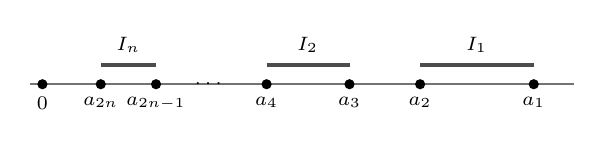
\begin{tikzpicture}[
  x=0.78cm,
  y=0.72cm,
  every node/.style={font=\scriptsize},
  axis/.style={black!55, line width=0.55pt},
  point/.style={circle, fill=black, inner sep=1.3pt},
  interval/.style={black!70, line width=1.2pt}
]
  \draw[axis] (-0.2,0) -- (8.65,0);

  \foreach \x/\lab in {
    0/$0$,
    0.95/a_{2n},
    1.85/a_{2n-1},
    3.65/a_4,
    5.00/a_3,
    6.15/a_2,
    8.00/a_1
  } {
    \node[point] at (\x,0) {};
    \node[below] at (\x,-0.05) {$\lab$};
  }

  \draw[interval] (0.95,0.34) -- (1.85,0.34);
  \draw[interval] (3.65,0.34) -- (5.00,0.34);
  \draw[interval] (6.15,0.34) -- (8.00,0.34);

  \node[above] at (1.40,0.38) {$I_n$};
  \node[above] at (4.32,0.38) {$I_2$};
  \node[above] at (7.07,0.38) {$I_1$};

  \node at (2.70,0) {$\cdots$};
\end{tikzpicture}

  \caption{The intervals $I_j=[a_{2j},a_{2j-1}]$ are disjoint inside $(0,a_1)$.}
  \label{fig:alternating-series-intervals}
\end{figure}

\begin{corollary} \label{cor:alternating-series-test} \hlt{Alternating Series Test}\\
Suppose $\abs{c_1}\geq\abs{c_2}\geq\abs{c_3}\geq\cdots$, the signs alternate, and $c_n\to0$. Then $\sum c_n$ converges.
\begin{proof}
After shifting indices to start at $0$ if desired, apply Theorem \ref{thm:dirichlet-test-series} with $a_n=(-1)^{n+1}$ and $b_n=\abs{c_n}$.\\
\hlt{Structural Commentary}: Alternation gives bounded sums; decreasing magnitudes damp them.\\
\hlt{Key Insight}: Alternating convergence is Dirichlet convergence in its simplest form.
\end{proof}
\end{corollary}

\begin{perspective} \label{per:alternating-series-interval-picture} \hlt{Alternating Partial Sums as Nested Control}\\
The interval picture explains the boundedness in Corollary \ref{cor:alternating-series-test}: the even partial sums collect disjoint lengths inside a fixed interval, while the odd partial sums differ from the even ones by the next term, which tends to $0$.
\end{perspective}

\begin{definition} \label{def:absolute-and-nonabsolute-convergence} \hlt{Absolute and Nonabsolute Convergence}\\
The series $\sum a_n$ \hlt{converges absolutely} if $\sum\abs{a_n}$ converges.\\
If $\sum a_n$ converges but $\sum\abs{a_n}$ diverges, then $\sum a_n$ converges \hlt{nonabsolutely}.
\end{definition}

\begin{theorem} \label{thm:absolute-convergence-implies-convergence} \hlt{Absolute Convergence Implies Convergence}\\
If $\sum a_n$ converges absolutely, then $\sum a_n$ converges.
\begin{proof}
For $m\geq n$, $\abs{\sum\limits_{k=n}^{m}a_k}\leq\sum\limits_{k=n}^{m}\abs{a_k}$. Apply Theorem \ref{thm:series-cauchy-criterion} to $\sum\abs{a_n}$.\\
\hlt{Structural Commentary}: Absolute convergence removes cancellation from the convergence question.\\
\hlt{Key Insight}: Small absolute tails force small signed or complex tails.
\end{proof}
\end{theorem}

\begin{theorem} \label{thm:linearity-of-convergent-series} \hlt{Addition and Scalar Multiplication of Series}\\
If $\sum a_n=A$ and $\sum b_n=B$, then $\sum(a_n+b_n)=A+B$ and $\sum ca_n=cA$ for every fixed scalar $c$.
\begin{proof}
Apply Theorem \ref{thm:complex-sequence-limit-algebra} to the corresponding partial sums.\\
\hlt{Structural Commentary}: Linearity of convergent series is just limit algebra for partial sums.\\
\hlt{Key Insight}: Add series by adding their partial-sum sequences.
\end{proof}
\end{theorem}

\begin{definition} \label{def:cauchy-product-of-series} \hlt{Cauchy Product}\\
Given $\sum a_n$, $\sum b_n$, define $c_n\defeq\sum\limits_{k=0}^{n}a_kb_{n-k}$, $(n=0,1,2,\ldots)$. Series $\sum c_n$ is \hlt{Cauchy product} of given series.
\end{definition}

\begin{figure}[H]
  \centering
  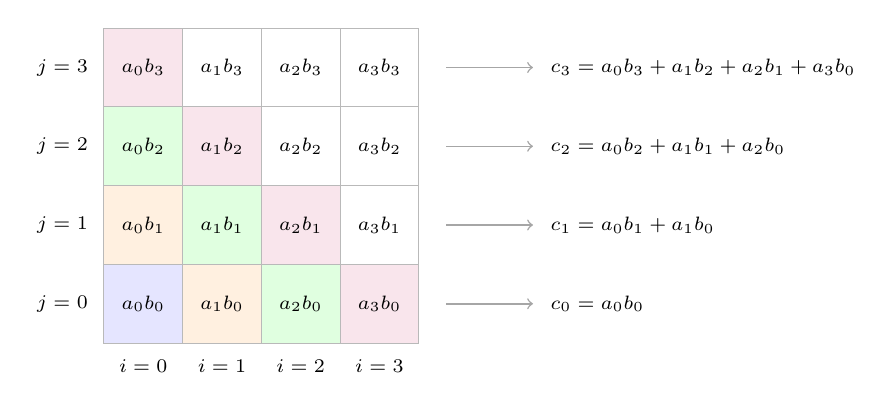
\begin{tikzpicture}[
  every node/.style={font=\scriptsize},
  cell/.style={draw=gray!55, line width=0.35pt},
  diagA/.style={fill=blue!10},
  diagB/.style={fill=orange!12},
  diagC/.style={fill=green!12},
  diagD/.style={fill=purple!10},
  arrow/.style={->, gray!70, line width=0.55pt}
]
  \foreach \i in {0,1,2,3} {
    \foreach \j in {0,1,2,3} {
      \pgfmathtruncatemacro{\diagindex}{\i+\j}
      \ifnum\diagindex=0
        \path[diagA] (\i,\j) rectangle ++(1,1);
      \fi
      \ifnum\diagindex=1
        \path[diagB] (\i,\j) rectangle ++(1,1);
      \fi
      \ifnum\diagindex=2
        \path[diagC] (\i,\j) rectangle ++(1,1);
      \fi
      \ifnum\diagindex=3
        \path[diagD] (\i,\j) rectangle ++(1,1);
      \fi
      \draw[cell] (\i,\j) rectangle ++(1,1);
      \node at (\i+0.5,\j+0.5) {$a_{\i}b_{\j}$};
    }
  }

  \foreach \i in {0,1,2,3} {
    \node[below] at (\i+0.5,-0.08) {$i=\i$};
    \node[left] at (-0.08,\i+0.5) {$j=\i$};
  }

  \draw[arrow] (4.35,0.5) -- (5.45,0.5);
  \node[right, align=left] at (5.55,0.5) {$c_0=a_0b_0$};

  \draw[arrow] (4.35,1.5) -- (5.45,1.5);
  \node[right, align=left] at (5.55,1.5) {$c_1=a_0b_1+a_1b_0$};

  \draw[arrow] (4.35,2.5) -- (5.45,2.5);
  \node[right, align=left] at (5.55,2.5) {$c_2=a_0b_2+a_1b_1+a_2b_0$};

  \draw[arrow] (4.35,3.5) -- (5.45,3.5);
  \node[right, align=left] at (5.55,3.5) {$c_3=a_0b_3+a_1b_2+a_2b_1+a_3b_0$};

\end{tikzpicture}

  \caption{Diagonal sums of $(a_i b_j)$ form the Cauchy product; finite rectangular sums are order-free.}
  \label{fig:cauchy-product-diagonals}
\end{figure}

\begin{perspective} \label{per:cauchy-product-diagonal-ordering} \hlt{Diagonal Ordering in a Product}\\
$c_n$ is the diagonal sum of the products $a_i b_j$ with $i+j=n$. Absolute convergence, as in Theorems \ref{thm:mertens-cauchy-product} and \ref{thm:absolute-convergence-rearrangements}, keeps the value independent of the accumulation order.
\end{perspective}

\begin{theorem} \label{thm:mertens-cauchy-product} \hlt{Mertens' Theorem for Cauchy Products}\\
Suppose $\sum a_n$ converges absolutely, $\sum a_n=A$, $\sum b_n=B$, and $c_n=\sum\limits_{k=0}^{n}a_kb_{n-k}$. Then $\sum\limits_{n=0}^{\infty}c_n=AB$.
\begin{proof}
Let $A_n,B_n,C_n$ be the partial sums and set $\beta_n\defeq B_n-B$.\\
Then $C_n=A_nB+\gamma_n$, and $\gamma_n\defeq a_0\beta_n+a_1\beta_{n-1}+\cdots+a_n\beta_0$. Since $A_nB\to AB$, it suffices to show $\gamma_n\to0$.\\
Put $\alpha\defeq\sum\abs{a_n}$. If $\abs{\beta_j}\leq\varepsilon$ for $j\geq N$, then $\abs{\gamma_n}\leq \abs{\beta_0a_n+\cdots+\beta_Na_{n-N}}+\varepsilon\alpha$.\\
Let $n\to\infty$ with $N$ fixed. The first term tends to $0$, so $\limsup\abs{\gamma_n}\leq\varepsilon\alpha$; let $\varepsilon\downarrow0$.\\
\hlt{Structural Commentary}: Absolute convergence of one factor controls the convolution error.\\
\hlt{Key Insight}: One absolute factor makes the Cauchy product converge to $AB$.
\end{proof}
\end{theorem}

\begin{definition} \label{def:series-rearrangement} \hlt{Rearrangement of a Series}\\
If $(k_n)$ lists each positive integer exactly once and $a'_n\defeq a_{k_n}$, then $\sum a'_n$ is a \hlt{rearrangement} of $\sum a_n$.
\end{definition}

\begin{theorem} \label{thm:riemann-rearrangement-theorem} \hlt{Riemann Rearrangement Theorem}\\
If real $\sum a_n$ converges nonabsolutely and $-\infty\leq\alpha\leq\beta\leq\infty$,\\
then some rearrangement has partial sums $s'_n$ with $\liminf\limits_{n\to\infty}s'_n=\alpha$ and $\limsup\limits_{n\to\infty}s'_n=\beta$.
\begin{proof}
Write $a_n=p_n-q_n$, where $p_n=\max(a_n,0)$ and $q_n=\max(-a_n,0)$. Since $\sum a_n$ converges but not absolutely, $\sum p_n=\sum q_n=+\infty$, and $p_n,q_n\to0$. List the positive nonzero $p_n$ as $P_1,P_2,\ldots$ and the positive nonzero $q_n$ as $Q_1,Q_2,\ldots$, preserving their original orders.\\
Choose finite numbers $\ell_N<u_N$ with $\ell_N\to\alpha$ and $u_N\to\beta$ in the extended sense. Starting from partial sum $0$, add unused $P$ terms until the sum is $>u_N$, then add unused terms $-Q$ until the sum is $<\ell_N$; repeat for $N=1,2,\ldots$. Divergence of both positive series makes each stopping time finite, and the alternating stages use every nonzero positive and negative term eventually. Insert zero terms anywhere.\\
After the $N$th upward crossing, the partial sum lies between $u_N$ and $u_N+P_j$ for the next positive term used; after the downward crossing, it lies between $\ell_N-Q_j$ and $\ell_N$ for the next negative term used. Since $P_j,Q_j\to0$, these overshoots vanish. Hence subsequences of partial sums approach the upper targets and lower targets, while all later partial sums stay within vanishing error of $[\ell_N,u_N]$. Therefore $\liminf s'_n=\alpha$ and $\limsup s'_n=\beta$.\\
\hlt{Structural Commentary}: Conditional convergence leaves enough mass to steer partial sums.\\
\hlt{Key Insight}: Vanishing terms make the steering increasingly precise.
\end{proof}
\end{theorem}

\begin{theorem} \label{thm:absolute-convergence-rearrangements} \hlt{Absolutely Convergent Series Are Rearrangement-Invariant}\\
Every rearrangement of an absolutely convergent complex series converges to the same sum.
\begin{proof}
Let $s_n,s'_n$ be the original and rearranged partial sums.\\
Given $\varepsilon>0$, choose $N$ so that $\sum_{i=N}^{m}\abs{a_i}\leq\varepsilon$ for $m\geq N$, then choose $p$ so $a_1,\ldots,a_N$ occur among $a'_1,\ldots,a'_p$.\\
For $n>p$, $s_n-s'_n$ uses only tail terms, hence $\abs{s_n-s'_n}\leq\varepsilon$. Thus $s'_n$ has the same limit as $s_n$.\\
\hlt{Structural Commentary}: Absolute tails control any finite reordering of the remaining terms.\\
\hlt{Key Insight}: Absolute convergence is exactly the protection needed against rearrangement.
\end{proof}
\end{theorem}

\begin{definition} \label{def:absolute-summation-over-countable-set} \hlt{Absolute Summation over Countable Sets}\\
Let $X$ be countable, $f:X\to\C$, and $g:\N\to X$ be a bijection, $g_n\defeq g(n)$.\\
If $\sum\limits_{n=1}^{\infty}\abs{f(g_n)}<\infty$, then $\sum\limits_{x\in X}f(x)$ is \hlt{absolutely convergent}, and $\sum\limits_{x\in X}f(x)\defeq\sum\limits_{n=1}^{\infty}f(g_n)$.
\end{definition}

\begin{theorem} \label{thm:absolute-countable-sums-well-defined} \hlt{Countable Sums Are Order-Free Under Absolute Convergence}\\
Let $X,Y$ be countable, $f:X\to\C$ be absolutely summable, and $h:Y\to X$ be a bijection.\\
Then $f\circ h$ is absolutely summable and $\sum\limits_{y\in Y}f(h(y))=\sum\limits_{x\in X}f(x)$.\\
In particular, a countable absolutely convergent sum is independent of the enumeration.
\begin{proof}
Let $g:\N\to X$ and $k:\N\to Y$ be enumerations, and set $\sigma\defeq g^{-1}\circ h\circ k:\N\to\N$.\\
Then $\sigma$ is a bijection and $h(k_n)=g_{\sigma(n)}$. Hence $\sum\limits_{n=1}^{\infty}\abs{f(h(k_n))} =\sum\limits_{n=1}^{\infty}\abs{f(g_{\sigma(n)})}<\infty$.\\
Thus $\sum\limits_{y\in Y}f(h(y)) =\sum\limits_{n=1}^{\infty}f(g_{\sigma(n)}) =\sum\limits_{n=1}^{\infty}f(g_n) =\sum\limits_{x\in X}f(x)$, where the middle equality is Theorem \ref{thm:absolute-convergence-rearrangements}.\\
Taking $Y=\N$ and $h$ to be any enumeration of $X$ gives enumeration independence.\\
\hlt{Structural Commentary}: Absolute convergence turns an enumeration into harmless bookkeeping.\\
\hlt{Key Insight}: Once absolute tails are controlled, the order of a countable listing no longer changes the sum.
\end{proof}
\end{theorem}

\begin{theorem} \label{thm:fubini-countable-absolute-series} \hlt{Fubini for Absolutely Summable Arrays}\\
Let $a_{mn}\in\C$ and suppose $L\defeq\sum\limits_{(m,n)\in\N\times\N}\abs{a_{mn}}<\infty$. Then each row and column is absolutely summable.\\
With $r_m\defeq\sum\limits_{n=1}^{\infty}a_{mn}$ and $c_n\defeq\sum\limits_{m=1}^{\infty}a_{mn}$, the row-total and column-total series are absolutely convergent,\\
where $\sum\limits_{m=1}^{\infty}\abs{r_m}<\infty$; $\sum\limits_{n=1}^{\infty}\abs{c_n}<\infty$, and $\sum\limits_{m=1}^{\infty}r_m =\sum\limits_{(m,n)\in\N\times\N}a_{mn} =\sum\limits_{n=1}^{\infty}c_n$.
\begin{proof}
For finite $F\subseteq\N\times\N$, $\sum_{(m,n)\in F}\abs{a_{mn}}\leq L$. Hence each row and column has bounded absolute partial sums, so rows and columns converge absolutely by Theorem \ref{thm:nonnegative-series-bounded-partial-sums}.\\
Moreover, for $M\geq1$, $\sum\limits_{m=1}^{M}\abs{r_m} \leq \sum\limits_{m=1}^{M}\sum\limits_{n=1}^{\infty}\abs{a_{mn}} =\lim\limits_{N\to\infty}\sum\limits_{m=1}^{M}\sum\limits_{n=1}^{N}\abs{a_{mn}} \leq L$, so $\sum\limits_m\abs{r_m}<\infty$.\\
Similarly $\sum\limits_n\abs{c_n}<\infty$. Let $\varepsilon>0$. Choose finite $F\subseteq\N\times\N$ with $\sum\limits_{(m,n)\in(\N\times\N)\setminus F}\abs{a_{mn}}<\varepsilon$, and choose a rectangle $R=\{1,\ldots,M\}\times\{1,\ldots,N\}\supseteq F$. The full sum, row-iterated sum, and column-iterated sum each differ from $\sum\limits_{(m,n)\in R}a_{mn}$ by at most $\sum\limits_{(m,n)\in(\N\times\N)\setminus R}\abs{a_{mn}}\leq\varepsilon$. Let $\varepsilon\downarrow0$.\\
\hlt{Structural Commentary}: Finite rectangles plus absolute tails justify Fubini.\\
\hlt{Key Insight}: Double sums can be rearranged only after the entire array is absolutely summable.
\end{proof}
\end{theorem}

\begin{method} \label{meth:series-proof-patterns-source-todo}\label{meth:series-proof-patterns} \hlt{Series Proof Patterns}
\begin{enumerate}[label=(\roman*)]
\setlength{\itemsep}{0pt}
\item \hlt{Partial sums}: translate every assertion about $\sum a_n$ into an assertion about $s_n=\sum_{k=1}^{n}a_k$.
\item \hlt{Cauchy tails}: prove convergence by estimating $\abs{\sum_{k=n}^{m}a_k}$ for $m\geq n$.
\item \hlt{Nonnegative terms}: replace convergence by boundedness of partial sums.
\item \hlt{Comparison}: dominate only the tail; finitely many early terms are irrelevant.
\item \hlt{Absolute convergence}: use $\sum\abs{a_n}$ when cancellation should not matter.
\item \hlt{Countable index sets}: choose a bijection $g:\N\to X$; use Theorem \ref{thm:absolute-countable-sums-well-defined} so $\sum_{x\in X}a_x$ is independent of $g$.
\item \hlt{Double sums}: prove identities on $R_{M,N}\defeq\{1,\ldots,M\}\times\{1,\ldots,N\}$; pass to $\infty$ arrays (Theorem \ref{thm:fubini-countable-absolute-series}).
\item \hlt{Conditional convergence}: order matters; use summation by parts or rearrangements.
\end{enumerate}
\hlt{Key Insight}: Series arguments are sequence arguments with special notation for tails.
\end{method}
